As we will see later, using the Finite Element method to solve problems involves computing integrals which are more often than not too complex to be computed analytically/exactly. We will then need to compute them numerically.

[wiki] In essence, 
the basic problem in numerical integration is to compute an approximate solution to a definite integral
\[
\int_a^b f(x) dx
\]
to a given degree of accuracy.
This problem has been widely studied and we know that 
if $f(x)$ is a smooth function, and the domain of integration is bounded, there are many methods for approximating the integral to the desired precision.

There are several reasons for carrying out numerical integration.
\begin{itemize}
\item The integrand $f(x)$ may be known only at certain points, such as obtained by sampling. Some embedded systems and other computer applications may need numerical integration for this reason.
\item A formula for the integrand may be known, but it may be difficult or impossible to find an antiderivative that is an elementary function. An example of such an integrand is $f(x)=exp(-x^2)$, the antiderivative of which (the error function, times a constant) cannot be written in elementary form.
\item It may be possible to find an antiderivative symbolically, but it may be easier to compute a numerical approximation than to compute the antiderivative. That may be the case if the antiderivative is given as an infinite series or product, or if its evaluation requires a special function that is not available.
\end{itemize}

%-----------------------------
\subsubsection{in 1D - theory}

The simplest method of this type is to let the interpolating function be a constant function (a polynomial of degree zero) that passes through the point $((a+b)/2, f((a+b)/2))$.

This is called the midpoint rule \index{midpoint rule} or rectangle rule. \index{rectangle rule}
\[
\int_a^b f(x)dx \simeq (b-a) f(\frac{a+b}{2})
\]

\improvement[inline]{insert here figure}

The interpolating function may be a straight line (an affine function, i.e. a polynomial of degree 1)
passing through the points $(a, f(a))$ and $(b, f(b))$.

This is called the trapezoidal rule. \index{trapezoidal rule} 
\[
\int_a^b f(x)dx \simeq (b-a) \frac{f(a)+f(b)}{2}
\]

\improvement[inline]{insert here figure}

For either one of these rules, we can make a more accurate approximation by breaking up the interval [a, b] into some number n of subintervals, computing an approximation for each subinterval, then adding up all the results. This is called a composite rule, extended rule, or iterated rule. For example, the composite trapezoidal rule can be stated as

\[
\int_a^b f(x)dx \simeq \frac{b-a}{n} \left( \frac{f(a)}{2}  
+\sum_{k=1}^{n-1} f(a+k\frac{b-a}{n})
   +\frac{f(b)}{2} \right)
\]

where the subintervals have the form $[kh,(k+1)h]$, with $h=(b-a)/n$ and $k=0,1,2,\dots,n-1$.


\begin{center}
a)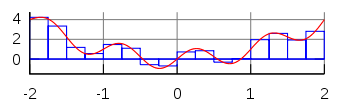
\includegraphics[width=7cm]{images/quadrature/int1}
b)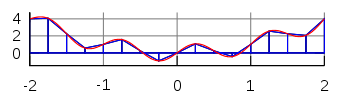
\includegraphics[width=7cm]{images/quadrature/int2}\\
The interval $[-2,2]$ is broken into 16 sub-intervals. The blue lines correspond to the 
approximation of the red curve by means of a) the midpoint rule,  b) the trapezoidal rule.
\end{center}

There are several algorithms for numerical integration (also commonly called 'numerical quadrature', or
simply 'quadrature') \index{quadrature}.
Interpolation with polynomials evaluated at equally spaced points in $[a,b]$
yields the Newton–Cotes formulas, of which the rectangle rule and the trapezoidal rule are examples. \index{Newton-Cotes}
If we allow the intervals between interpolation points to vary, we find another group of quadrature formulas, such as 
the Gauss(ian) quadrature formulas. \index{Gauss quadrature}
A Gaussian quadrature rule is typically more accurate than a Newton–Cotes rule, 
which requires the same number of function evaluations, if the integrand is smooth 
(i.e., if it is sufficiently differentiable).


An $n-$point Gaussian quadrature rule, named after Carl Friedrich Gauss, is a quadrature rule constructed
to yield an exact result for polynomials of degree $2n-1$ or less by a suitable choice of the points $x_i$
and weights $w_i$ for $i=1,\dots,n$.

The domain of integration for such a rule is conventionally taken as $[-1,1]$, so the rule is stated as
\[
\int_{-1}^{+1} f(x) dx = \sum_{i_q=1}^n w_{i_q} f(x_{i_q})
\]
In this formula the $x_{i_q}$ coordinate is 
the $i$-th root of the Legendre polynomial $P_n(x)$. \index{Legendre polynomial}

It is important to note that a Gaussian quadrature will only produce good results if the function $f(x)$
is well approximated by a polynomial function within the range $[-1,1]$.
As a consequence, the method is not, for example, suitable for functions with singularities.

\begin{center}
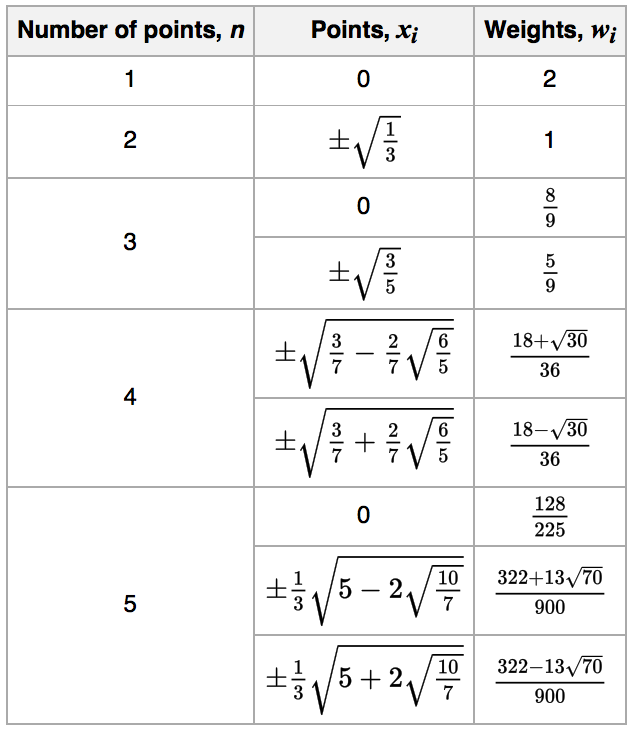
\includegraphics[width=5.cm]{images/quadrature/gq2}\\
Gauss-Legendre points and their weights.
\end{center}

\begin{tabular}{lllll}
\hline
n & $x_{iq}$ & $w_{iq}$ & $x_{iq}$ (approx) & $w_{iq}$ (approx) \\
\hline\hline
1 & 0 & 2 & 0 & 2 \\
\hline
2 & $\pm \sqrt{1/3}$ & 1  & $\pm$0.577350269189626 & 1 \\
\hline
3 & 0 & 8/9 & 0 & 0.888888888888889 \\
  & $\pm\sqrt{3/5}$  & 5/9  & $\pm$0.774596669241483 & 0.555555555555556 \\
\hline
4 & $\pm\sqrt{\frac{3}{7} - \frac{2}{7}\sqrt{6/5}}$  & $\frac{18+\sqrt{30}}{36}$ & $\pm$0.339981043584856 & 0.652145154862546 \\
  & $\pm\sqrt{\frac{3}{7} + \frac{2}{7}\sqrt{6/5}}$  & $\frac{18-\sqrt{30}}{36}$ & $\pm$0.861136311594053 & 0.347854845137454 \\
\hline
5 & 0 & 128/225 & 0 & 0.568888888888889 \\
  & $\pm\frac{1}{3}\sqrt{5-2\sqrt{\frac{10}{7}}}$  & $\frac{322+13\sqrt{70}}{900}$ & $\pm$0.538469310105683 & 0.478628670499366 \\
  & $\pm\frac{1}{3}\sqrt{5+2\sqrt{\frac{10}{7}}}$  & $\frac{322-13\sqrt{70}}{900}$ & $\pm$0.906179845938664 & 0.236926885056189 \\
\hline
6 & ?& ?& $\pm$0.23861 91860 83197 & 0.46791 39345 72691 \\
  & ?& ?& $\pm$0.66120 93864 66265 & 0.36076 15730 48139 \\
  & ?& ?& $\pm$0.93246 95142 03152 & 0.17132 44923 79170 \\
\hline
\end{tabular}



As shown in the above table, it can be shown that the weight values must fulfill the following condition:
\begin{equation}
\sum_{i_q} w_{i_q}=2 \label{gq23}
\end{equation}
and it is worth noting that all quadrature point coordinates are symmetrical around the origin.

Since most quadrature formula are only valid on a specific interval, we now must address the problem 
of their use outside of such intervals. The solution turns out to be quite simple: one 
must carry out a change of variables from the interval $[a,b]$ to $[-1,1]$.

We then consider the reduced coordinate $r\in[-1,1]$ such that 
\[
r=\frac{2}{b-a}(x-a)-1 
\]
This relationship can be reversed such that when $r$ is known, its equivalent coordinate 
$x\in[a,b]$ can be computed:
\[
x=\frac{b-a}{2}(1+r)+a
\]
From this it follows that
\[
dx=\frac{b-a}{2}dr
\]
and then 
\[
\int_a^b f(x) dx  = \frac{b-a}{2} \int_{-1}^{+1} f(r) dr \simeq 
\frac{b-a}{2} \sum_{i_q=1}^n w_{i_q} f(r_{i_q})
\]

%--------------------
\subsubsection{in 1D - examples}

\paragraph{example 1}

Since we know how to carry out any required change of variables, we choose for simplicity 
$a=-1$, $b=+1$.
Let us take for example $f(x)=\pi$. Then we can compute the integral of this function 
over the interval $[a,b]$ exactly:
\[
I=\int_{-1}^{+1} f(x) dx = \pi \int_{-1}^{+1}dx  = 2 \pi
\]
We can now use a Gauss-Legendre formula to compute this same integral:
\[
I_{gq}=\int_{-1}^{+1} f(x) dx 
= \sum_{i_q=1}^{n_q} w_{i_q} f(x_{i_q}) 
= \sum_{i_q=1}^{n_q} w_{i_q} \pi
= \pi \underbrace{\sum_{i_q=1}^{n_q} w_{i_q} }_{=2}
= 2 \pi
\]
where we have used the property of the weight values of Eq.(\ref{gq23}).
Since the actual number of points was never specified, this result is valid for all 
quadrature rules.


\paragraph{example 2}

Let us now take $f(x)=m x+ p$ and repeat the same exercise:
\[
I=\int_{-1}^{+1} f(x) dx = \int_{-1}^{+1} (mx+p) dx  =  [\frac{1}{2} m x^2 + p x ]_{-1}^{+1} =2p
\]
\[
I_{gq}=\int_{-1}^{+1} f(x) dx 
\!= \sum_{i_q=1}^{n_q} w_{i_q} f(x_{i_q}) 
\!= \sum_{i_q=1}^{n_q} w_{i_q} (m x_{i_q} + p)  
\!= m \underbrace{\sum_{i_q=1}^{n_q} w_{i_q} x_{i_q}}_{=0}  + p \underbrace{\sum_{i_q=1}^{n_q} w_{i_q}}_{=2}  = 2p
\]
since the quadrature points are symmetric w.r.t. to zero on the x-axis.
Once again the quadrature is able to compute the exact value of this integral: this makes sense since 
an $n$-point rule exactly integrates a $2n-1$ order polynomial such that a 1 point quadrature exactly 
integrates a first order polynomial like the one above.



\paragraph{example 3}

Let us now take $f(x)=x^2$. We have 
\[
I=\int_{-1}^{+1} f(x) dx = \int_{-1}^{+1} x^2 dx  =  [\frac{1}{3}x^3 ]_{-1}^{+1} =  \frac{2}{3} 
\]
and 
\[
I_{gq}=\int_{-1}^{+1} f(x) dx 
\!= \sum_{i_q=1}^{n_q} w_{i_q} f(x_{i_q}) 
\!= \sum_{i_q=1}^{n_q} w_{i_q} x_{i_q}^2 
\]

\begin{itemize}
\item $n_q=1$: $x_{iq}^{(1)}=0$, $w_{i_q}=2$. $I_{gq}=0$
\item $n_q=2$: $x_{q}^{(1)}=-1/\sqrt{3}$, $x_{q}^{(2)}=1/\sqrt{3}$, $w_{q}^{(1)}=w_{q}^{(2)}=1$. $I_{gq}=\frac{2}{3}$
\item It also works $\forall n_q>2$ !
\end{itemize}

%-----------------------------
\subsubsection{in 2D/3D - theory}


Let us now turn to a two-dimensional integral of the form
\[
I=\int_{-1}^{+1} \int_{-1}^{+1} f(x,y) dx dy
\]
The equivalent Gaussian quadrature writes:
\[
I_{gq}
\simeq \sum_{i_q=1}^{n_q}\sum_{j_q}^{n_q} f(x_{i_q},y_{j_q}) w_{i_q} w_{j_q}
\]

%----------------------------------------
\subsubsection{quadrature on triangles}

Quadrature rules for triangles can be found in Dunavant, 1985 \cite{duna85}.
The following ones are identical to those in the {\sl ip\_triangle.m} 
file of the MILAMIN code \cite{daks08}.

{\small
\[
\begin{array}{ccccccc}
\hline
&r_q & s_q & w_q \\ 
\hline\hline
iq=1& 1/3 & 1/3 & 1/2\\
\hline
iq=1 & 1/6 & 1/6 & 1/6 \\
iq=2 & 2/3 & 1/6 & 1/6 \\
iq=3 & 1/6 & 2/3 & 1/6 \\
\hline
iq=1&1/3 & 1/3 & -27/96\\
iq=2&0.6 & 0.2 &  25/96\\
iq=3&0.2 & 0.6 &  25/96\\
iq=4&0.2 & 0.2 &  25/96\\
\hline
iq=1& 1-2g_1 & g_1 & w_1/2  &  0.108103018168070 & 0.44594849091596  &   \\
iq=2& g_1 & 1-2g_1 & w_1/2  &  0.445948490915965 & 0.108103018168070 &   \\
iq=3& g_1 & g_1    & w_1/2  &  0.445948490915965 & 0.445948490915965 &   \\
iq=4& 1-2g_2 & g_2 & w_2/2  &  0.816847572980459 & 0.091576213509771 &   \\
iq=5& g_2 & 1-2g_2 & w_2/2  &  0.091576213509771 & 0.816847572980459 &   \\
iq=6& g_2 & g_2    & w_2/2  &  0.091576213509771 & 0.091576213509771 &   \\
\hline
iq=1&&&&0.091576213509771 &  0.091576213509771    &    0.109951743655322/2.0 \\ 
iq=2&&&&0.816847572980459 &  0.091576213509771    &    0.109951743655322/2.0 \\
iq=3&&&&0.091576213509771 &  0.816847572980459    &    0.109951743655322/2.0 \\
iq=4&&&&0.445948490915965 &  0.445948490915965    &    0.223381589678011/2.0 \\
iq=5&&&&0.108103018168070 &  0.445948490915965    &    0.223381589678011/2.0 \\
iq=6&&&&0.445948490915965 &  0.108103018168070    &    0.223381589678011/2.0 \\
\hline
iq=1 &&&&0.1012865073235 &  0.1012865073235  &     0.0629695902724 \\
iq=2 &&&&0.7974269853531 &  0.1012865073235  &     0.0629695902724 \\
iq=3 &&&&0.1012865073235 &  0.7974269853531  &     0.0629695902724 \\
iq=4 &&&&0.4701420641051 &  0.0597158717898  &     0.0661970763942 \\
iq=5 &&&&0.4701420641051 &  0.4701420641051  &     0.0661970763942 \\
iq=6 &&&&0.0597158717898 &  0.4701420641051  &     0.0661970763942 \\
iq=7 &&&&0.3333333333333 &  0.3333333333333  &     0.1125000000000 \\
\hline
iq=1&&&& 5.01426509658179E-01&  2.49286745170910E-01 &   5.83931378631895E-02 \\ 
iq=2&&&& 2.49286745170910E-01&  5.01426509658179E-01 &   5.83931378631895E-02 \\ 
iq=3&&&& 2.49286745170910E-01&  2.49286745170910E-01 &   5.83931378631895E-02 \\ 
iq=4&&&& 8.73821971016996E-01&  6.30890144915020E-02 &   2.54224531851035E-02 \\ 
iq=5&&&& 6.30890144915020E-02&  8.73821971016996E-01 &   2.54224531851035E-02 \\ 
iq=6&&&& 6.30890144915020E-02&  6.30890144915020E-02 &   2.54224531851035E-02 \\ 
iq=7&&&& 5.31450498448170E-02&  3.10352451033784E-01 &   4.14255378091870E-02 \\ 
iq=8&&&& 6.36502499121399E-01&  5.31450498448170E-02 &   4.14255378091870E-02 \\ 
iq=9&&&& 3.10352451033784E-01&  6.36502499121399E-01 &   4.14255378091870E-02 \\ 
iq=10&&&& 5.31450498448170E-02&  6.36502499121399E-01 &   4.14255378091870E-02 \\ 
iq=11&&&& 6.36502499121399E-01&  3.10352451033784E-01 &   4.14255378091870E-02 \\ 
iq=12&&&& 3.10352451033784E-01&  5.31450498448170E-02 &   4.14255378091870E-02 \\ 
\hline
\end{array}
\]
}

where
\[ 
g_1 = \left(8-\sqrt{10} + \sqrt{38-44\sqrt{2/5}}\right)/18
\qquad
g_2 = \left(8-\sqrt{10} - \sqrt{38-44\sqrt{2/5}}\right)/18
\]
\[
w_1 = \left(620+\sqrt{213125-53320\sqrt{10}}\right)/3720
\qquad
w_2 = \left(620-\sqrt{213125-53320\sqrt{10}}\right)/3720
\]


      


%----------------------------------------
\subsubsection{quadrature on tetrahedra}

\begin{remark}
In what follows the coefficients in the tables are not the reduced coordinates
of the quadratue points but the coefficients corresponding to the 4 nodes.
\end{remark}

Quadrature rules on tetrahedra take the form:
\[
\int\int\int_{el} f(x,y,z) dxdydz = V_{el} \sum_{iq=1}^{nqel} w_{iq} f(\xi^{iq}_1,\xi^{iq}_2,\xi^{iq}_3,\xi^{iq}_4) 
\]
or, that is to say:
\[
\int\int\int_{el} f(x,y,z) dxdydz = \sum_{iq=1}^{nqel} (w_{iq}V_{el}) f(\xi^{iq}_1,\xi^{iq}_2,\xi^{iq}_3,\xi^{iq}_4) 
\]
with in our case $V_{el}=1/6$.

In the literature it can be found that a one point quadrature is characterised by 
\[
w_{iq}=1 \quad\quad\quad \xi^{iq}_1=\xi^{iq}_2=\xi^{iq}_3=\xi^{iq}_4=0.25
\]
i.e, the coordinates of the single point are given by:
\[
x_{iq}=\sum_{i=1}^4 \xi_i^{iq} x_i = \frac{1}{4} (x_1+x_2+x_3+x_4)
\]
Same for $y$ and $z$ coordinates. 

A four-point quadrature rule is characterised by $w_{iq}=V_el*0.25=1/24\simeq 04166666666666667$ and 

\begin{tabular}{lcccc}
 & $\xi_1$ & $\xi_2$ & $\xi_3$ & $\xi_4$ \\
iq=1 & 0.585410196624969 & 0.138196601125011 & 0.138196601125011 & 0.138196601125011 \\
iq=2 & 0.138196601125011 & 0.585410196624969 & 0.138196601125011 & 0.138196601125011 \\
iq=3 & 0.138196601125011 & 0.138196601125011 & 0.585410196624969 & 0.138196601125011 \\
iq=4 & 0.138196601125011 & 0.138196601125011 & 0.138196601125011 & 0.585410196624969 \\
\end{tabular}

We then have:
\[
r_{iq}=\sum_{i=1}^4 \xi_i^{iq} x_i 
= (\xi_1^{iq},\xi_2^{iq},\xi_3^{iq},\xi_4^{iq})\cdot(r_1,r_2,r_3,r_4) 
= (\xi_1^{iq},\xi_2^{iq},\xi_3^{iq},\xi_4^{iq})\cdot(0,1,0,0) 
= \xi_2^{iq}
\]
\[
s_{iq}=\sum_{i=1}^4 \xi_i^{iq} y_i 
= (\xi_1^{iq},\xi_2^{iq},\xi_3^{iq},\xi_4^{iq})\cdot(s_1,s_2,s_3,s_4) 
= (\xi_1^{iq},\xi_2^{iq},\xi_3^{iq},\xi_4^{iq})\cdot(0,0,1,0) 
= \xi_3^{iq}
\]
\[
t_{iq}=\sum_{i=1}^4 \xi_i^{iq} z_i 
= (\xi_1^{iq},\xi_2^{iq},\xi_3^{iq},\xi_4^{iq})\cdot(t_1,t_2,t_3,t_4) 
= (\xi_1^{iq},\xi_2^{iq},\xi_3^{iq},\xi_4^{iq})\cdot(0,0,0,1) 
= \xi_4^{iq}
\]
Finally:

\[
\begin{array}{ccccc}
     & r_q & s_q & t_q  & w_q \\
iq=1 & 0.138196601125011 & 0.138196601125011 & 0.138196601125011 & 0.04166666666666667\\
iq=2 & 0.585410196624969 & 0.138196601125011 & 0.138196601125011 & 0.04166666666666667\\
iq=3 & 0.138196601125011 & 0.585410196624969 & 0.138196601125011 & 0.04166666666666667\\
iq=4 & 0.138196601125011 & 0.138196601125011 & 0.585410196624969 & 0.04166666666666667\\
\end{array}
\]


%------------------------------------------
\subsubsection{The Gauss-Lobatto approach}

All what we have seen above falls under the Gauss-Legendre quadrature method. There is however another 
somewhat common quadrature method: the Gauss-Lobatto  quadrature. \index{Gauss-Lobatto}.
It is similar to Gaussian quadrature with the following  important differences:
1) There are integration points in the interval but they also always include the end points of the integration interval;
2) It is accurate for polynomials up to degree $2n-3$, where $n$ is the number of integration points.

In 1D, it reads:
\[
\int_{-1}^{+1} f(x) dx = \frac{2}{n(n-1)} [f(-1)+f(1)] + \sum_{i=2}^{n-1} w_i f(x_i) 
\]
The locations and weights of the integration points are as follows:

\begin{center}
\begin{tabular}{lllll}
\hline
n & $x_{iq}$ & $w_{iq}$ & $x_{iq}$ (approx) & $w_{iq}$ (approx) \\
\hline\hline
3 & 0 & 4/3 & & \\
  & $\pm 1$ & 1/3 & &  \\
\hline
4 & $\pm\sqrt{\frac{1}{5}}$ & 5/6 & & \\
  & $\pm 1$ & 1/6 & & \\
\hline
5 & 0 & 32/45 & & \\
  & $\pm\sqrt{\frac{3}{7}}$ & 49/90 & & \\
  & $\pm 1$ & 1/10 & & \\
\hline
6 & $\pm\sqrt{\frac{1}{3} -\frac{2\sqrt{7}}{21}}$ & $\frac{14+\sqrt{7}}{30}$ & & \\
  & $\pm\sqrt{\frac{1}{3} +\frac{2\sqrt{7}}{21}}$ & $\frac{14-\sqrt{7}}{30}$ & & \\
  & $\pm 1$ & 1/15 \\
\hline
\end{tabular}
\end{center}

 






